\section{Research Hypotheses and Contributions}
\label{sec:hypotheses}

We hypothesize that the integration of data derived from non-invasive wearable sensors, coupled with the application of machine learning methodologies to connect physiological and biomechanical aspects, holds the potential to formulate objective, precise, and automated approaches for assessing fitness and anticipating the onset of fatigue in sport horses. In the following, we address the stated research questions and propose the following corresponding hypotheses, alongside their main contributions, as concisely shown in Figure \ref{fig:summary}:

\begin{figure}[htb]
\centering
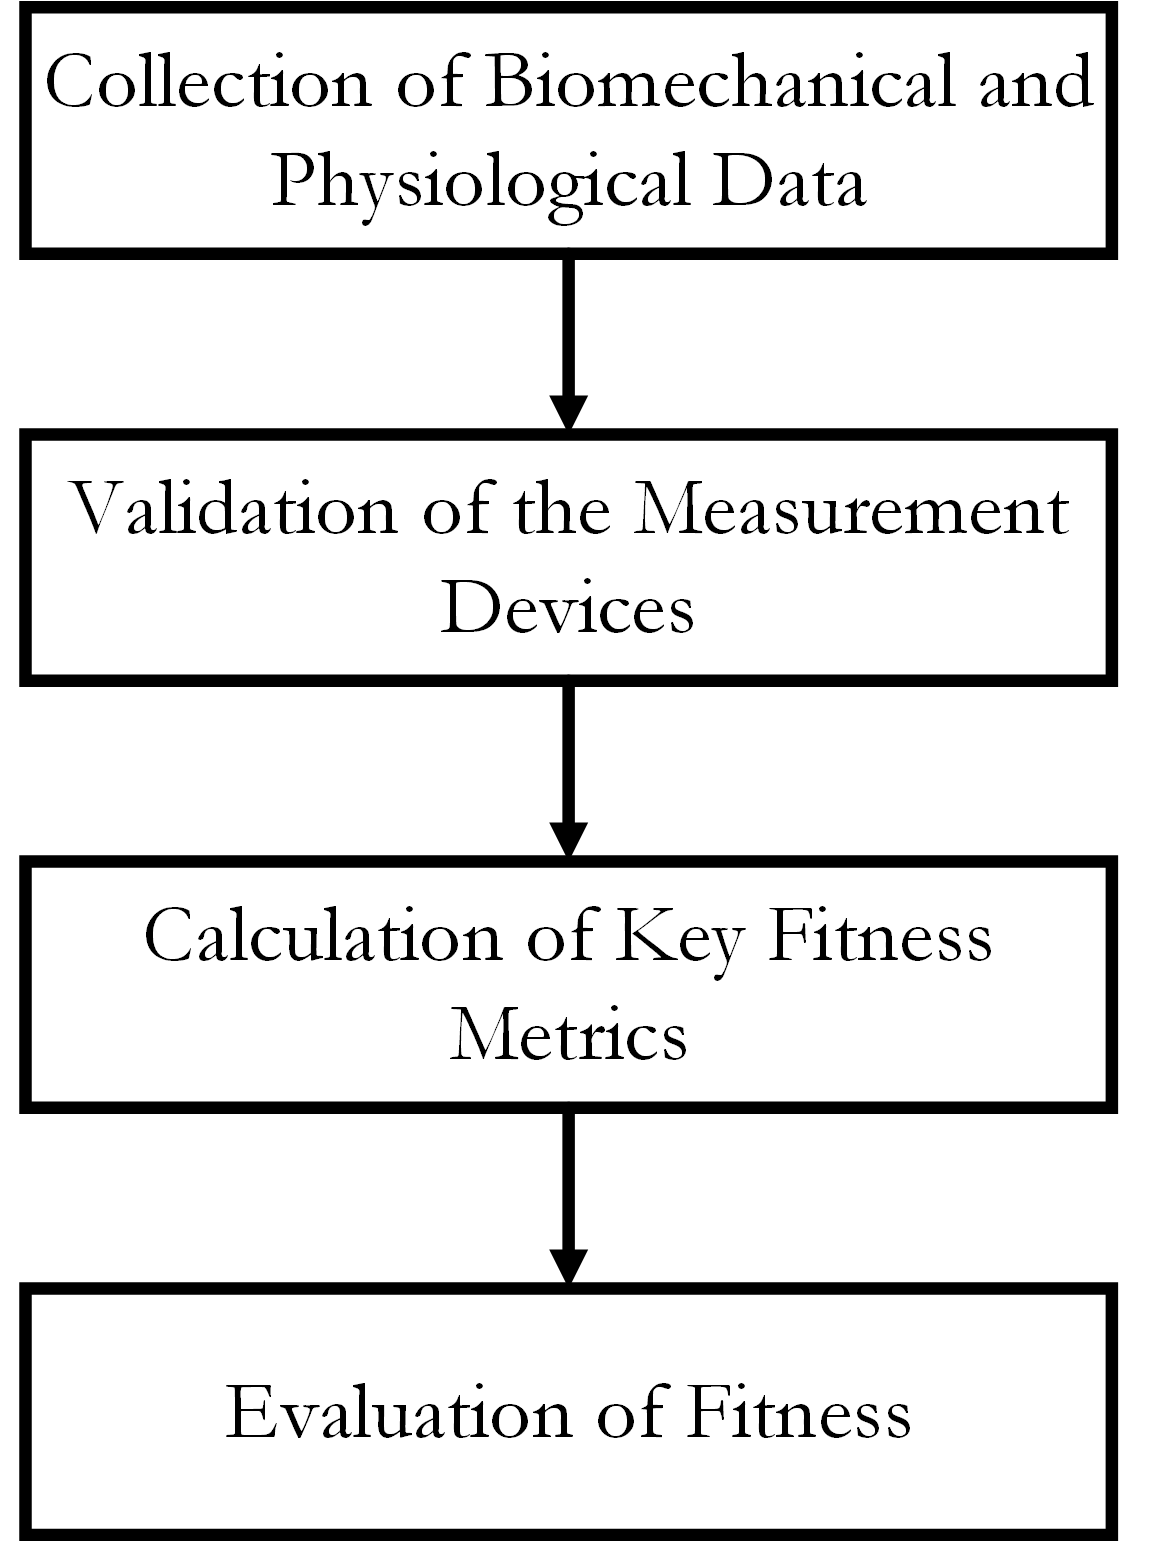
\includegraphics[width=.35\linewidth]{../tables/Naamloos.png}
\caption{Summary of thesis proposed hypotheses}
\label{fig:summary}
\end{figure}

\vspace{0.25cm}

\noindent\textbf{\large Hypothesis 1:} We hypothesize that by developing machine learning models using data from wearable sensors, the key fitness parameters can be calculated. This hypothesis is approached in five steps to answer \textbf{Research Questions 1, 2, and 3},

    \begin{enumerate}
        \item Review the literature to identify the key parameters that impact fitness
\item Collecting high-quality data of sport horses gait using wearable sensors
\item Developing mathematical/machine learning models for calculating the identified key parameters
\item Investigating the accuracy of the developed models
\item Investigating the reliability of wearable sensors used in the calculation of the identified key parameters compared to the traditional methods
    \end{enumerate} 

\noindent \textbf{\large Contributions to Hypothesis 1:} 

\vspace{0.1cm}

Throughout Chapters 3 to 5, this thesis presents three studies that focus on fitness parameters. Each chapter commences with an extensive review of relevant literature. Subsequently, the objective of the chapter is determined based on the recurring themes and significance found in the literature. The subsequent sections of each chapter are dedicated to exploring effective and adaptable methodologies for evaluating the selected parameter. 

\vspace{0.25cm}

\noindent\textbf{Chapter 3: Fitness Metrics - Gait Events}

\noindent Step-related parameters, such as stride duration, are key parameters in fitness assessment. Therefore, we try to develop a detection model for hoof-on and hoof-off events and compare it with traditional methods. This chapter highlights the importance of speed as a crucial fitness variable, and it explores different methods to calculate and analyze it in depth. This chapter has been published as:

\begin{itemize}
\item[]\begin{footnotesize}\textit{Darbandi, H., Braganca, F. S., van der Zwaag, B. J., \& Havinga, P. (2022). Accurate horse gait event estimation using an inertial sensor mounted on different body locations. 2022 IEEE International Conference on Smart Computing (SMARTCOMP). https://doi.org/10.1109/smartcomp55677.2022.00076} \end{footnotesize}
\end{itemize}

\noindent\textbf{Chapter 4: Fitness Metrics - Gait Biomechanics}

\noindent Pelvis angles are used as a gold standard to detect fit-to-compete horses. Therefore, we try to measure them using wearable sensors. By validating the \gls{imu} for measurement of pelvis angles, we assure its usability for other body joint angles and displacements, or gait biomechanical parameters. In this chapter, the significance of joint angles and body displacements is emphasized, and methods for their calculation are investigated. This chapter has been published as:
\begin{itemize}
    \item[]\begin{footnotesize}\textit{Darbandi, H., Braganca, F. S., Smit, I. H., Voskamp, J., \& Havinga, P. In Comparing two methods of estimating pelvis roll using IMU sensors and optical motion capture (Poster). International Conference on Equine Exercise Physiology.  Uppsala. Retrieved 2023, from 10.13140/RG.2.2.14252.13440}\end{footnotesize}\end{itemize}


\noindent\textbf{Chapter 5: Fitness Metrics - Spatio-temporal Parameters}

\noindent One of the key parameters mentioned several times in the literature is speed. Therefore, we aim to develop an estimation model for speed and compare it with traditional methods. Within this chapter, the focus lies on emphasizing the relevance of gait events as an important category of fitness parameters. Subsequently, the chapter thoroughly examines the most efficient and accurate methods available to calculate and analyze these gait events in-depth, providing a comprehensive understanding of their importance. This chapter has been published as:


\begin{itemize}
    \item[] \begin{footnotesize}\textit{Darbandi, H., Serra Bragança, F., van der Zwaag, B. J., Voskamp, J., Gmel, A. I., Haraldsdóttir, E. H., \& Havinga, P. (2021). Using different combinations of body-mounted IMU sensors to estimate speed of horses—a machine learning approach. Sensors, 21(3), 798. https://doi.org/10.3390/s21030798}  \end{footnotesize}\end{itemize}
    
\vspace{0.5cm}



\noindent\textbf{\large Hypothesis 2:} We hypothesize that by using the fitness parameters models as the input, fitness can be defined and evaluated. This hypothesis is approached in three steps to answer \textbf{Research Question 4 and 5},


    \begin{enumerate}
\item Collecting high-quality data from sport horses during standardized exercise tasks
\item Developing predictive models using identified parameters and machine learning for assessing fitness and fatigue
\item Optimizing the models in terms of practicality, usability, and efficiency
    \end{enumerate} 

\noindent \textbf{\large Contributions to Hypothesis 2:} 

\vspace{0.1cm}

Building upon the collected data presented in Chapter 2, and the models established for the calculation and estimation of fitness-related parameters in Chapters 3 to 5, Chapters 6 to 8 will focus on the development and training of more advanced models, specifically designed for fitness assessment. This chapter has been published as:

\vspace{.25cm}

\noindent\textbf{Chapter 6: Fitness Assessment - Rider or No Rider? That's The Question!}

\noindent The fitness of sport horses has been measured while ridden. Therefore, it is important to monitor the ridden horse for probable fatigue occurrence. We want to know if there is any impact on performance and find important parameters directly from the wearable sensors' signals. This chapter centers on the impact of riders on horse biomechanics and performance. Here, we focus on significant parameters among those that were introduced in Chapters 3 to 5, exploring their susceptibility to rider influence. Additionally, we introduce a binary classification approach aimed at determining whether a horse is ridden or not, leveraging the signals from the \gls{imu}s. This chapter has been published as:

\noindent\begin{itemize}
\item[]\begin{footnotesize}\textit{Darbandi, H., \& Havinga, P. (2022). A machine learning approach to analyze rider’s effects on horse gait using on-body inertial sensors. 2022 IEEE International Conference on Pervasive Computing and Communications Workshops and Other Affiliated Events (PerCom Workshops). https://doi.org/10.1109/percomworkshops53856.2022.9767228}\end{footnotesize}\end{itemize}

\noindent\textbf{Chapter 7: Fitness Assessment: Ready for Exercise?}

\noindent To assess the differences in the values of the parameters between normal and fatigued sport horses, we create a model based on the identified parameters to classify if the horse is fatigued or not using the physiological definition of fatigue. This chapter aims to automatically detect fatigue in sport horses using a minimum number of \gls{imu}s. Machine learning models are developed to identify key fatigue indicators, leading to accurate classification models. The importance of different fitness metrics is examined for fatigue detection. This chapter has been published as:

\begin{itemize}
\item[]\begin{footnotesize} \textit{
Darbandi, H., Munsters, C., Parmentier, J., \& Havinga, P. (2023). Detecting fatigue of sport horses with biomechanical gait features using inertial sensors. PLOS ONE, 18(4). https://doi.org/10.1371/journal.pone.0284554 }
\end{footnotesize} \end{itemize}

\noindent\textbf{Chapter 8: Fitness Assessment: Evaluation of Fatigue}

\noindent To quantify the fatigue in sport horses, we develop a model to estimate \gls{lac}, an important physiological indicator of fatigue, based on the data from wearable sensors. This chapter proposes a non-invasive approach by combining biomechanical and physiological aspects of sport horses to measure their fatigue during exercise. This chapter has been published as:
\begin{itemize}
\item[]\begin{footnotesize} \textit{Darbandi, H., Munsters, C., \& Havinga, P. (2024). A Non-Invasive Lactate Estimation Using Wearable Sensors for Remote Fatigue Assessment in Horses. 2024 IEEE International Conference on Pervasive Computing and Communications Workshops and other Affiliated Events. 10.1109/PerComWorkshops59983.2024.10503247}
\end{footnotesize} 
\end{itemize}